\subsection{Análisis de resultados}

Sumado a la comparación entre distintas implementaciones del
\textsc{Disjoint-Set} en esta sección mostraremos segmentaciones resultantes de
ejecutar el algoritmo con distintos parámetros. También se ofrecen adjuntos
tres videos dónde se varía cada uno de los parámetros mientras se fijan los
otros dos\footnote{Dado que la forma en la que elegimos los colores no resultó
estable respecto de variar $\sigma$ el video dónde se lo varía podría resultar
molesto para personas con fotosensibildad.}.

\begin{figure}[h]
	\centering
	\begin{subfigure}{0.4\linewidth}
		
\includegraphics[width=\linewidth]{segmentation/entradas-posta/sintetico}
		\caption{Entrada}
	\end{subfigure}
	\begin{subfigure}{0.4\linewidth}
		\includegraphics[width=\linewidth]{segmentation/salidas/{0.8.sintetico.png.500.1000}.png}
		\caption{Segmentación}
	\end{subfigure}
	\caption{$\sigma = 0.8,\ k = 500,\ g = 1000$.}
\end{figure}

Una buena segmentación es un concepto difícil de definir, dado que depende el
nivel de granularidad deseado ciertos segmentos pueden resultar útiles o no
(ventanas en edificios, ojos en personas, letras individuales en una hoja,
etc). Cómo nuestro algoritmo sólo percibe la intensidad de cada píxel se pierde
información propia del color en la transformación que nos genera casos de error
que podrían salvarse de otro modo.

\subsubsection{Errores esperables}

Escojer un bien el valor de $\sigma$ resulta importante para eliminar ciertas
imperfecciones. Valores de entre $0.4$ t $0.8$ fueron los que utilizamos para
ver los resultados\footnote{Se puede correr \texttt{make ver\_todos} en
\texttt{segmentation} para ver los resultados con $\sigma = 0.8$, $k = 600$ y
sin pasada de simplificación. También se pueden pasar los valores como
parámetro en la forma \texttt{make BLUR=$\sigma$ K=$k$ MIN=$g$ ver\_todos}.}.

En las siguientes imágenes se pueden apreciar distintas segmentaciones de uno
de las imágenes que no pudimos encontrar un conjunto de parámetros que ofrezcan
una segmentación razonable. Dado que la evidente diferencia de color no se
traslada a la entrada en escala de grises. Puede observarse cómo el proceso de
simplificación mantiene algunos de los limites de la imagen original para
valores de $k$ muy bajos y cómo pu puede ser útil eliminar segmentos demasiado
chicos con esa técnica en lugar de elevar el $k$ perdiendo los segmentos del
insecto.

\begin{figure}[h]
	\centering
	\begin{subfigure}{0.4\linewidth}
		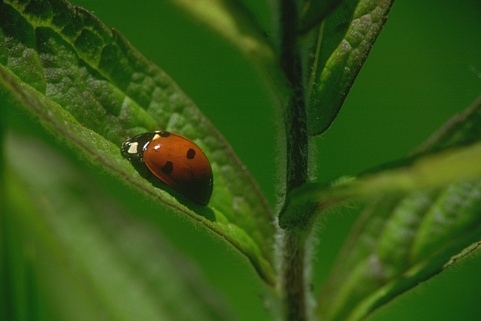
\includegraphics[width=\linewidth]{segmentation/entradas-posta/mariquita}
		\caption{Entrada}
	\end{subfigure}
	\begin{subfigure}{0.4\linewidth}
		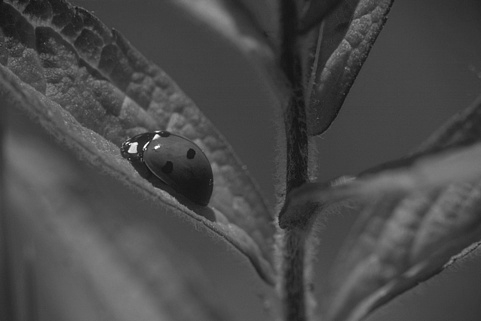
\includegraphics[width=\linewidth]{segmentation/informe/mariquita}
		\caption{Entrada en escala de grises}
	\end{subfigure}
	\begin{subfigure}{0.4\linewidth}
		\includegraphics[width=\linewidth]{segmentation/salidas/{0.0.mariquita.jpg.6000.-1}.png}
		\caption{$\sigma = 0,\ k = 6000$}
	\end{subfigure}
	\begin{subfigure}{0.4\linewidth}
		\includegraphics[width=\linewidth]{segmentation/salidas/{0.0.mariquita.jpg.0.1000}.png}
		\caption{$\sigma = 0,\ k = 0,\ g = 1000$}
	\end{subfigure}
	\begin{subfigure}{0.4\linewidth}
		\includegraphics[width=\linewidth]{segmentation/salidas/{0.0.mariquita.jpg.600.-1}.png}
		\caption{$\sigma = 0,\ k = 600$}
	\end{subfigure}
	\begin{subfigure}{0.4\linewidth}
		\includegraphics[width=\linewidth]{segmentation/salidas/{0.0.mariquita.jpg.600.1000}.png}
		\caption{$\sigma = 0,\ k = 600,\ g = 1000$}
	\end{subfigure}
	\caption{Distintas configuraciones con distintos tipos de error,
	aquellas que no especifican valores para $g$ no tuvieron paso de
	simplificación.}
\end{figure}

\clearpage

La importancia del desenfoque no es evidente en todas las imágenes, la
siguiente escena muestra un defecto que ocurre cuando las fotos tienen mucho
grano:

\begin{figure}[h]
	\centering
	\begin{subfigure}{0.3\linewidth}
		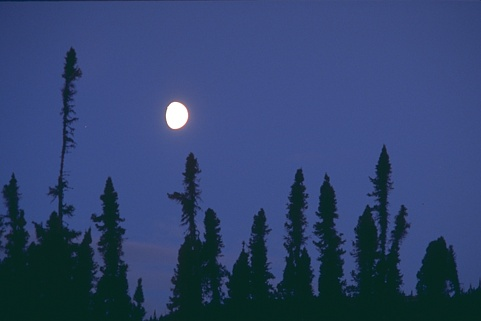
\includegraphics[width=\linewidth]{segmentation/entradas-posta/noche}
		\caption{Entrada}
	\end{subfigure}
	\begin{subfigure}{0.3\linewidth}
		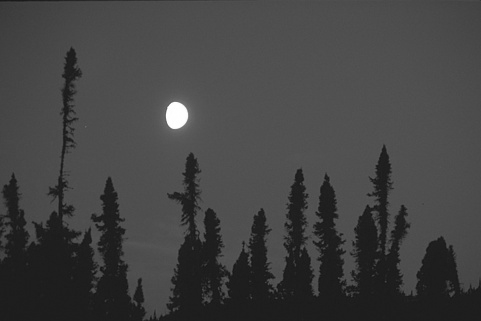
\includegraphics[width=\linewidth]{segmentation/informe/noche}
		\caption{Escala de grises}
	\end{subfigure}
	\begin{subfigure}{0.3\linewidth}
		\includegraphics[width=\linewidth]{segmentation/salidas/{0.0.noche.jpg.600.-1}.png}
		\caption{$\sigma = 0,\ k = 600$}
	\end{subfigure}
	\begin{subfigure}{0.3\linewidth}
		\includegraphics[width=\linewidth]{segmentation/salidas/{0.2.noche.jpg.600.-1}.png}
		\caption{$\sigma = 0.2,\ k = 0$}
	\end{subfigure}
	\begin{subfigure}{0.3\linewidth}
		\includegraphics[width=\linewidth]{segmentation/salidas/{0.4.noche.jpg.600.-1}.png}
		\caption{$\sigma = 0.4,\ k = 600$}
	\end{subfigure}
	\begin{subfigure}{0.3\linewidth}
		\includegraphics[width=\linewidth]{segmentation/salidas/{0.6.noche.jpg.600.-1}.png}
		\caption{$\sigma = 0.6,\ k = 600$}
	\end{subfigure}
	\begin{subfigure}{0.4\linewidth}
		\includegraphics[width=\linewidth]{segmentation/salidas/{0.8.noche.jpg.600.-1}.png}
		\caption{$\sigma = 0.8,\ k = 600$}
	\end{subfigure}
	\begin{subfigure}{0.4\linewidth}
		\includegraphics[width=\linewidth]{segmentation/salidas/{1.0.noche.jpg.600.-1}.png}
		\caption{$\sigma = 1,\ k = 600$}
	\end{subfigure}
	\caption{Segmentación de una escena simple con grano.}
\end{figure}

\clearpage

\subsubsection{Resultados favorables}

\begin{figure}[h]
	\centering
	\begin{subfigure}{0.3\linewidth}
		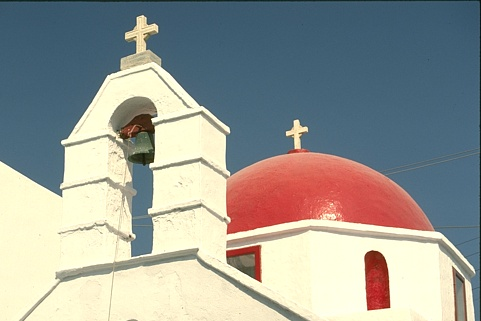
\includegraphics[width=\linewidth]{segmentation/entradas-posta/iglesia}
		\caption{Entrada}
	\end{subfigure}
	\begin{subfigure}{0.3\linewidth}
		\includegraphics[width=\linewidth]{segmentation/salidas/{0.8.iglesia.jpg.600.-1}.png}
		\caption{$\sigma = 0.8,\ k = 600$}
	\end{subfigure}
	\begin{subfigure}{0.3\linewidth}
		\includegraphics[width=\linewidth]{segmentation/salidas/{0.8.iglesia.jpg.600.1000}.png}
		\caption{$g = 1000$}
	\end{subfigure}
	\caption{Segmentacion de \texttt{iglesia.jpg}}
\end{figure}

\begin{figure}[h]
	\centering
	\begin{subfigure}{0.3\linewidth}
		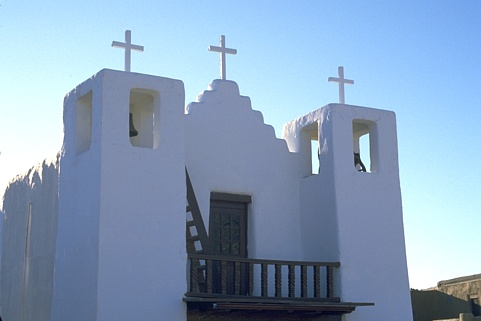
\includegraphics[width=\linewidth]{segmentation/entradas-posta/iglesia_2}
		\caption{Entrada}
	\end{subfigure}
	\begin{subfigure}{0.3\linewidth}
		\includegraphics[width=\linewidth]{segmentation/salidas/{0.8.iglesia_2.jpg.600.-1}.png}
		\caption{$\sigma = 0.8,\ k = 600$}
	\end{subfigure}
	\begin{subfigure}{0.3\linewidth}
		\includegraphics[width=\linewidth]{segmentation/salidas/{0.8.iglesia_2.jpg.600.1000}.png}
		\caption{$g = 1000$}
	\end{subfigure}
	\caption{Segmentacion de \texttt{iglesia\_2.jpg}}
\end{figure}

\begin{figure}[h]
	\centering
	\begin{subfigure}{0.3\linewidth}
		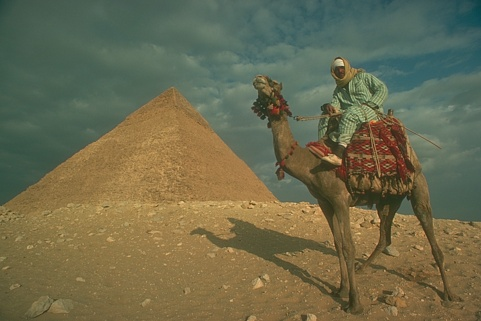
\includegraphics[width=\linewidth]{segmentation/entradas-posta/piramide_camello}
		\caption{Entrada}
	\end{subfigure}
	\begin{subfigure}{0.3\linewidth}
		\includegraphics[width=\linewidth]{segmentation/salidas/{0.8.piramide_camello.jpg.300.-1}.png}
		\caption{$\sigma = 0.8,\ k = 300$}
	\end{subfigure}
	\begin{subfigure}{0.3\linewidth}
		\includegraphics[width=\linewidth]{segmentation/salidas/{0.8.piramide_camello.jpg.300.1000}.png}
		\caption{$g = 1000$}
	\end{subfigure}
	\caption{Segmentacion de \texttt{piramide\_camello.jpg}}
\end{figure}

Cómo puede observarse, dado suficiente contraste el algoritmo genera
segmentaciones razonables, aunque por usar la 8-vecindad de cada píxel
construye pequeños segmentos en lugares quese ven cortados por una sombra.
